\chapter{Marco Te\'orico}

Este capitulo est\'a basado en el libro \textit{Diffusion MRI} \cite{Basser2009}
y en las clases del Doctor Michael L. Lipton \cite{Lipton2014} disponibles online. 
En caso de querer profundizar en alg\'un tema, por favor referirse a estos. 

\section{MRI}
Se denomina momento magn\'etico nuclear al momento magn\'etico que posee un 
\'atomo a causa del spin de sus protones y electrones. Cuando un momento 
magn\'etico $\mu$ es puesto dentro de un campo magn\'etico, comenzara a preceder 
alrededor de la direcci\'on de este \'ultimo siguiendo la frecuencia de Larmor: 

$$ \omega = \frac{d\theta}{dt} = gB $$

Donde $\omega$ es la velocidad angular, $g$ es la relaci\'on giromagn\'etica y 
$B$ es la fuerza del campo. A su vez, la cantidad de energ\'ia que posea el campo
determinara el \'angulo entre $\mu$ y el campo mientras sucede la precesi\'on. 
Esto quiere decir que dado un $B$ suficientemente grande es posible hacer que 
la precesi\'on suceda en la direcci\'on transversal del campo, lo cual permitir\'ia
medir $|\mu|$ simplemente poniendo una bobina en ese plano. Si uno realizara
el experimento notar\'ia que al apagar el campo, la se\~nal comienza a desvanecerse,
esto es porque el sistema comienza a perder energ\'ia provocando que el \'angulo
entre $\mu$ y el campo se achique. A este proceso se lo denomina relajaci\'on. \\

\begin{figure}[h!]

\begin{minipage}[b]{0.49\textwidth}
    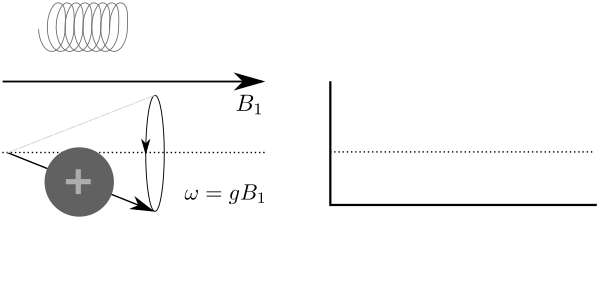
\includegraphics[width=\textwidth]{img/spin0.png}
    \caption{Spin sometido a un campo magn\'etico debil}
\end{minipage} ~ %add desired spacing between images, e. g. ~, \quad, \qquad, \hfill etc. %(or a blank line to force the subfigure onto a new line) 
\hfill
\begin{minipage}[b]{0.49\textwidth}
    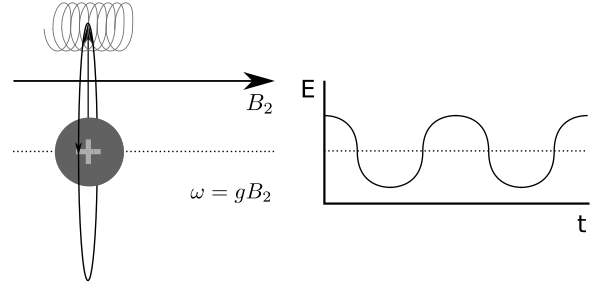
\includegraphics[width=\textwidth]{img/spin1.png}
    \caption{Resultado de aumentar el campo magn\'etico}
\end{minipage} ~ %add desired spacing between images, e. g. ~, \quad, \qquad, \hfill etc. %(or a blank line to force the subfigure onto a new line) 

\end{figure}

\vspace{0.1cm}
Vayamos ahora al plano m\'edico. El cuerpo est\'a compuesto por distintos 
tipos de tejidos, cada uno con su propia composici\'on qu\'imica, lo cual 
determina un momento magn\'etico distinto para cada uno de ellos, y por ende
un tiempo de relajaci\'on particular. Esto implica que al poner a un paciente
dentro de un campo magn\'etico, cada tejido comenzara a generar un momento 
en base a la poblaci\'on de protones que posea. Como ya fue dicho, para medir
el tiempo de relajaci\'on de estos es necesario primero llevar los momentos magn\'eticos
al plano transversal. El problema es que si uno intentara administrar energ\'ia al 
sistema simplemente aumentando la fuerza del campo magn\'etico terminar\'ia da\~nando
al paciente. Aqu\'i es donde se aprovecha la frecuencia de Larmor. Conociendo la
composici\'on qu\'imica de cada tejido es posible calcular su frecuencia angular.
Luego, mediante el efecto de resonancia es posible transmitir energ\'ia al 
sistema simplemente emitiendo ondas en esa misma frecuencia. \\

\begin{figure}[h!]
                                                                                                                        
\begin{minipage}[b]{0.49\textwidth}
    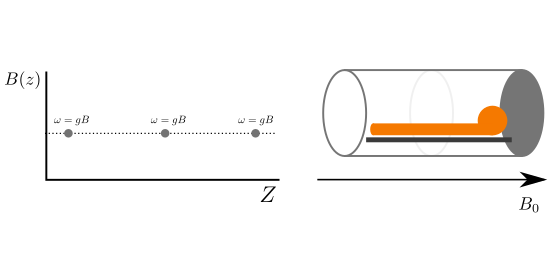
\includegraphics[width=\textwidth]{img/grad0.png}
    \caption{\small  Campo uniforme, todos los protones poseen la misma velocidad angular}
     \label{fig:unif}
\end{minipage} ~
\hfill
\begin{minipage}[b]{0.49\textwidth}
    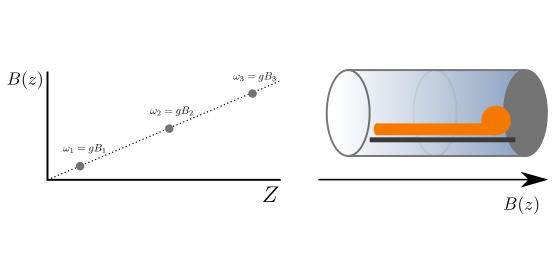
\includegraphics[width=\textwidth]{img/grad1.png}
    \caption{\small Campo gradiente, la velocidad angular de los protones var\'ia linealmente }
    \label{fig:grad}
\end{minipage} ~

\end{figure}  

\vspace{0.1cm}

Los resonadores magn\'eticos son dispositivos con la capacidad de generar 
campos y pulsos en diferentes frecuencias, en partocular todo resonador encendido
est\'a emitiendo constantemente un campo homog\'eneo $B_0$. 
El problema entonces es: c\'omo obtener el tiempo de relajaci\'on 
de un punto particular del cuerpo. Para esto es posible utilizar campos 
gradientes. Un campo gradiente es un campo que var\'ia su potencia linealmente
a lo largo de una direcci\'on, provocando que todas los protones a lo 
largo de esa direcci\'on var\'ien su frecuencia angular de manera predecible. 
Aplicando un campo gradiente $G_z$ en la direcci\'on $z$ (ver Fig. \ref{fig:grad})
sobre el paciente haremos que la velocidad en funci\'on de la posici\'on sea:
$\omega(z) = B_z(z) g$, esto nos asegurara que si aplicamos el pulso de RF a una
frecuencia de $B_z(z_o) g$, solo los protones que se encuentran en la posici\'on
$z=z_o$ comenzaran a resonar, por lo que estos ser\'an los \'unicos que generen un 
campo transversal. Cabe destacar que como no es posible generar un pulso con
exactamente la frecuencia deseada, tambi\'en resonaran los protones que se 
encuentren cerca, por lo que tendremos un intervalo $[z_o-\epsilon,z_o+\epsilon]$
resonando. A este proceso se lo denomina \textit{slice selection}. Podemos pensar 
el slice como una matriz de dos dimensiones sobre el eje $z$. Si ahora aplicamos
un campo gradiente $G_\psi$ en la direcci'on $y$, suceder\'a que todas las 
filas de nuestra matriz adquiriran diferentes velocidades angulares. Al apagar
$G_\psi$ todos los protones volveran a preceder respecto al campo $B_0$, pero
est\'a vez estaran desfasados por filas (ver Fig. \ref{fig:kspace}). Encendiendo
un tercer campo gradiente $G_\upsilon$ sobre la direcci\'on $x$ conseguiremos
que cada columna posea una frecuencia distinta y cada fila una fase distinta.
Repitiendo este procedimiento varias veces cambiando solo la intensidad de
$G_\psi$ podemos armar lo que se conoce como \textit{k-space}. El \textit{k-space}
es una imagen espacial temporal donde est\'an anotados los valores obtenidos para
cada potencia utilizada, en orden ascendente de potencia. El aplicar una
transformada de Fourier 3D a dicho espacio nos devolver\'a la imagen que
representa el contraste de cada tejido en el \textit{slice} seleccionado. \\

\begin{figure}[h!]
                                                                                                                        
\begin{minipage}[b]{\textwidth}
    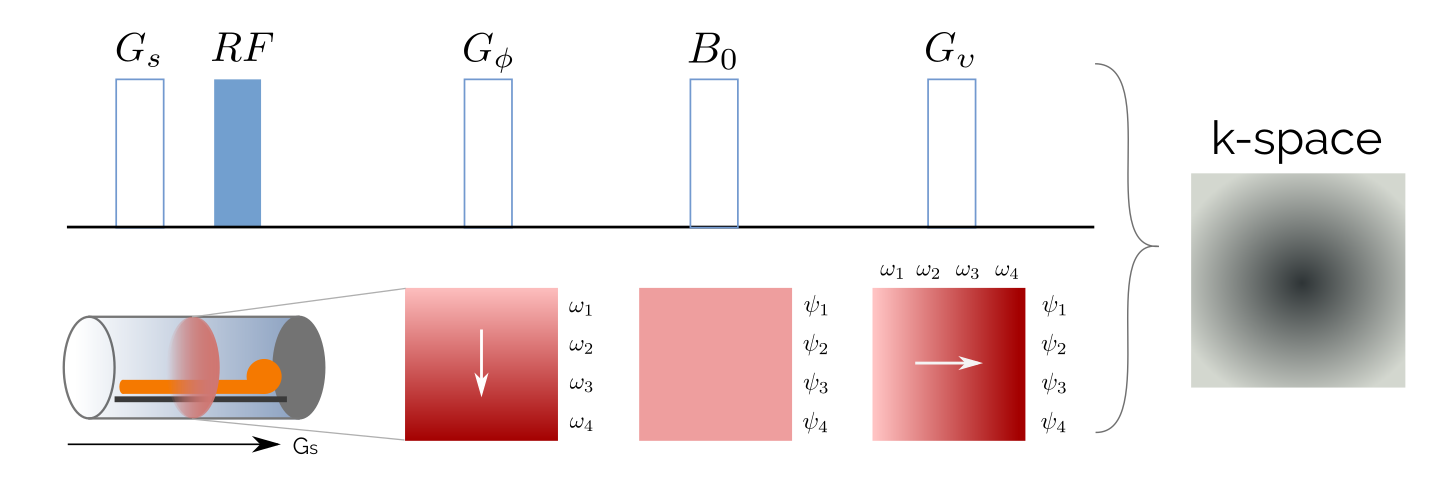
\includegraphics[width=\textwidth]{img/kspace.png}
    \caption{Resumen del proceso de adquisici\'on de im\'agenes en MRI}
    \label{fig:kspace}
\end{minipage} ~

\end{figure}  



\section{dMRI}

Las mol\'eculas dentro de un fluido en equilibrio no se encuentras est\'aticas,
sino que se mueven realizando un camino aleatorio. A este fen\'omeno se lo 
conoce con el nombre de difusi\'on. \\

Modificando la secuencia del resonador es posible medir la intensidad de 
difusi\'on que poseen distintos puntos dentro del cerebro. Por ej, si luego de
aplicar el pulso RF se agrega un campo gradiente $G_1=G_d$ durante un tiempo $\delta$
peque\~no pero de alta potencia, es posible generar un desfase entre los
spines de los protones. El aplicar $G_2=-G_d$ luego de $\Delta$ deber\'ia provocar
que los protones se vuelvan a alinear. Sin embargo, por estar sometidos al efecto
del movimiento Browniano, los protones se habr\'an movido, provocando que el campo
magn\'etico los alcance en distintas posiciones, y por ende afecte de distinta
manera su velocidad angular. Esto nos indica que si hay difusi\'on entonces habr\'a
un desfase en esa poblaci\'on de neutrones (ver Fig \ref{fig:dmri}).\\

Es importante entender que por limitaciones f\'isicas de los dispositivos es
imposible obtener la se\~nal producida por un solo prot\'on. En general lo que
se obtiene es la resultante de los momentos magn\'eticos de todos los protones
dentro de un espacio. Si todos los protones estuvieran precediendo a la misma
velocidad sobre el mismo plano, entonces la resultante m\'axima se obtiene si 
todos poseen la misma fase, esto es, todos se encuentran en la misma posici\'on 
al mismo tiempo. Gracias a esto es posible traducir la diferencia de fase
en p\'erdida de se\~nal. \\

\vspace{0.1cm}

\begin{figure}
                                                                                                                        
\begin{minipage}[b]{\textwidth}
    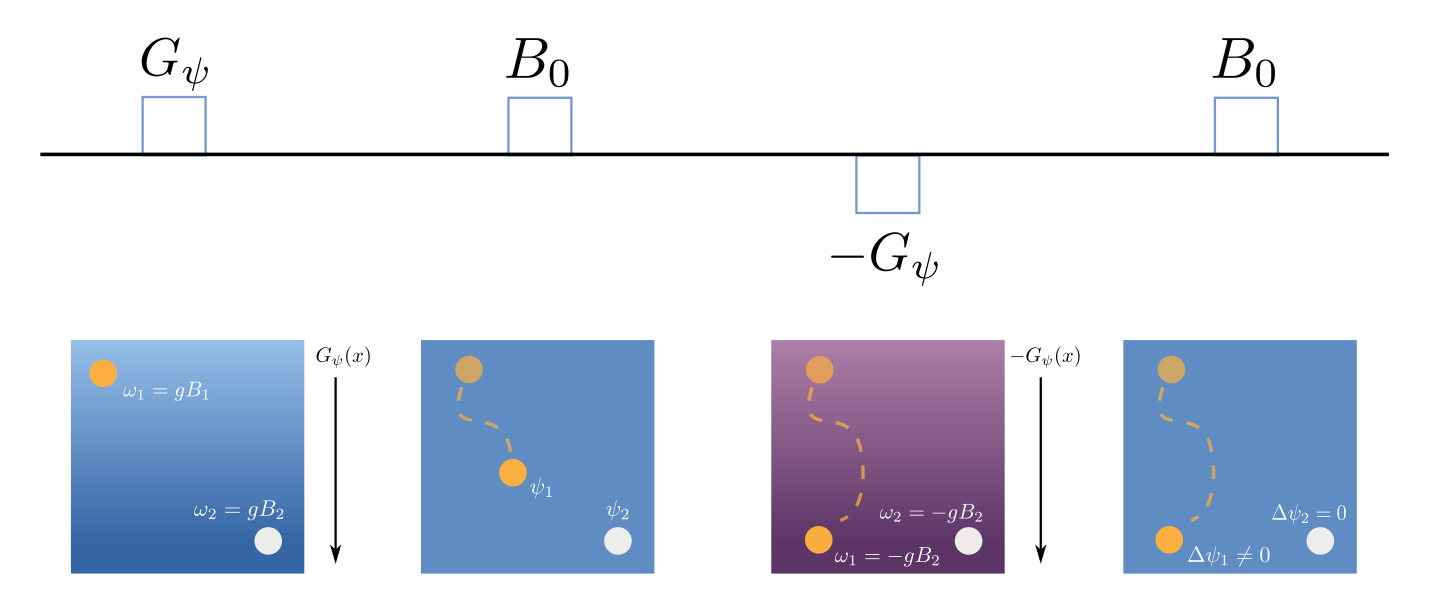
\includegraphics[width=\textwidth]{img/dmri.png}
    \caption{Modificar la secuencia permite medir la intensidad de difusi\'on}
    \label{fig:dmri}
\end{minipage} ~

\end{figure}  

\begin{wrapfigure}{r}{0.5\textwidth}
    \begin{center}
        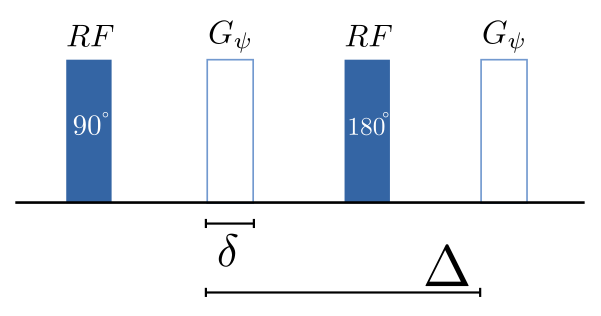
\includegraphics[width=0.4\textwidth]{img/fgp.png}
        \caption{Field Gradient Pulse}
        \label{fig:fgp}
    \end{center}
\end{wrapfigure}  

En 1965 Stejskal y Tanner \cite{Stejskal1965} cren una secuencia denominada 
\textit{Field Gradient Pulse} en la cual utilizan dos pulsos RF y un mismo campo
magn\'etico para caracterizar la difusi\'on (ver Figura \ref{fig:fgp}). Luego, 
asumiendo que el desplazamiento debido a la difusi\'on sigue una distribuci\'on 
normal demuestran que la relaci\'on entre la intensidad de difusi\'on y la perdida de
se\~nal puede ser modelada mediante la ecuaci\'on:

\vspace{0.3cm}

$$ E(b) = \frac{S(b)}{S_0} = e^{-b D} \label{eq:stejkal}$$
$$ b = -g^2 B^2 \delta^2 (\Delta^2 - \frac{\delta}{3}) $$

$E(b)$ es la atenuaci\'on de la se\~nal obtenida; $S_0$ es la se\~nal obtenida
sin utilizar gradientes de difusi\'on; $B$ es la intensidad del gradiente de
difusi\'on, $g$ es la relaci\'on giromagn\'etica;  $\delta$ es el tiempo que el
gradiente de difusi\'on est\'a encendido; $\Delta$ es el tiempo entre las 
activaciones del grediente y $D$ representa el coeficiente de difusi\'on.
La raz\'on por la cual se divide la se\~nal obtenida por $S_0$ es porque la
se\~nal en cada punto depende fuertemente de la densidad de protones que hay
en el mismo, si no ponderamos dicha densidad, es imposible comparar la intensidad
de difusi\'on en distintas regiones. \\

La ecuaci\'on de Stejskal y Tanner sienta las bases de lo que se conoce como 
\textit{Diffusion Tensor Imaging} (DTI). En esta t\'ecnica se mide la atenuaci\'on
de se\~nal en al menos seis direcciones y luego se aproxima el coeficiente de 
difusi\'on con un tensor de segundo orden. Un tensor es una matriz multidimensional 
asociado a una base, que posee una ley de transformaci\'on  para indicar  c\'omo
cambian los componentes del tensor al cambiar de base. En DTI el tensor que m\'as
se utiliza representa un elipsoide en $R^3$. La matriz que lo representa
es  sim\'etrica, por ello es que se necesitan tomar al menos seis adquisiciones: 

$$
    D =
    \begin{pmatrix}
             D_{xx} & D_{xy} & D_{xz} \\
             D_{xy} & D_{yy} & D_{yz} \\
             D_{xz} & D_{yz} & D_{zz}    
    \end{pmatrix}
$$

\vspace{0.1cm}

El problema con utilizar este es que no permite representar correctamente
el cruce de fibras dentro de cada voxel dado que las caracteriza con un solo
elipsoide.\\

En 1991 Callaghan et al \cite{Callaghan1991} desarrollan el \textit{q-space analysis}.
Comenzando desde la misma base que Stejskal y Tanner, demuestran que sin asumir un
modelo para la distribuci\'on de desplazamiento, pero tomando un $\delta$ chico,
se deriva la siguiente relaci\'on entre la se\~nal atenuada y una transformada de
Fourier:

$$E(q,t) =  \frac{S(q,t)}{S_0} = \int_{R^2}{p(r,t)e^{-2\pi i q r} dr} $$
$$ q = \frac{g \delta B}{2\pi} $$

Donde $q$ es una medida que relaciona $B$ con $\delta$; $t$ es el tiempo durante
el cual se mide la se\~nal; $p(r,t)$ es la densidad de probabilidad de que una
poblaci\'on de part\'iculas se desplace en direcci\'on $r$ durante ese tiempo $t$.\\

Una de las principales ventajas de \textit{q-space} sobre DTI es que no asume
ning\'un modelo a priori, esto permite definir distintos tipos de modelos para
$p(r,t)$ que caracterizan mejor el cruce de fibras. \textit{Spherical Harmonics}
\cite{Tuch2004} o \textit{Constrained Spherical Deconvolution} \cite{Tournier2004}.
son ejemplos de ello \\
